\documentclass[tikz,border=12pt]{standalone}
\usepackage[T1]{fontenc}
\usepackage{mathpazo}
\usepackage{amsmath,amssymb}
\usetikzlibrary{arrows.meta, positioning, calc, fit, patterns, decorations.pathreplacing}

\definecolor{stblue}{HTML}{7B97AD}
\definecolor{rwgold}{HTML}{B8995E}
\definecolor{sage}{HTML}{7A9A7E}
\definecolor{dkbrown}{HTML}{3D3530}
\definecolor{wmgray}{HTML}{7B7067}
\definecolor{cream}{HTML}{F9F6F0}
\definecolor{border}{HTML}{D4C9B8}
\definecolor{terracotta}{HTML}{C47A6A}
\definecolor{lavender}{HTML}{907EA0}

\begin{document}
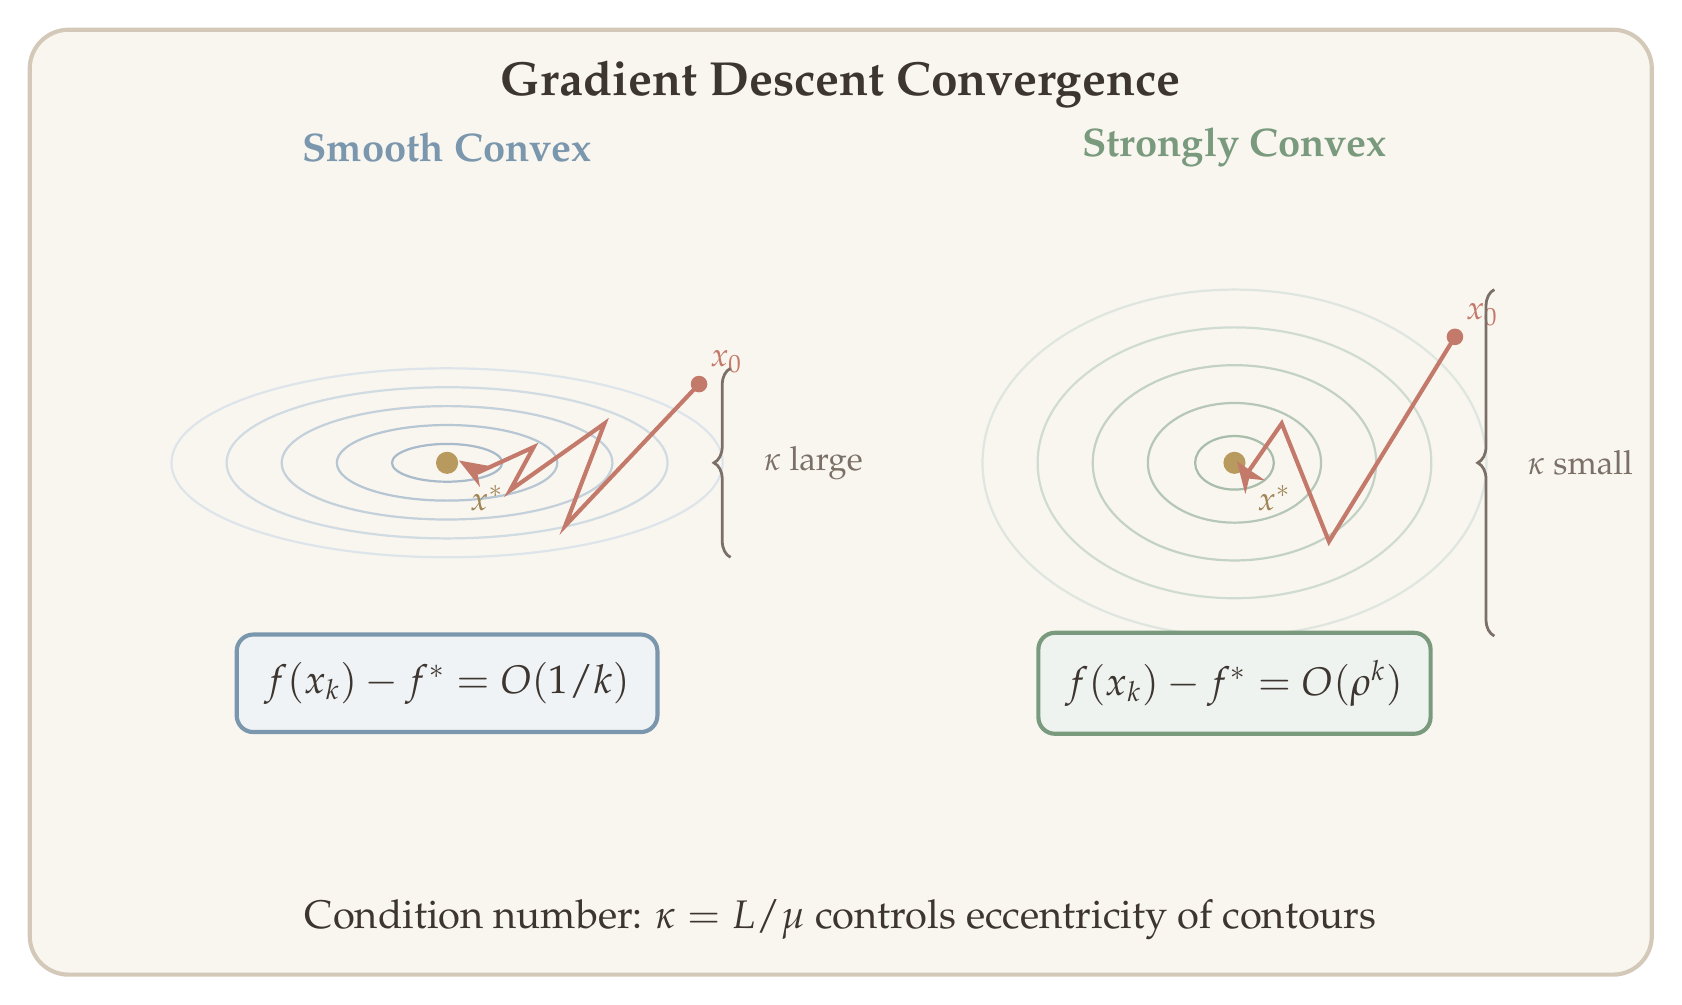
\begin{tikzpicture}[>={Stealth[length=4mm, width=3mm]}, line width=1.5pt]

% Background
\fill[cream, rounded corners=14pt] (-0.8,-3.5) rectangle (19.8,8.5);
\draw[border, line width=1.5pt, rounded corners=14pt] (-0.8,-3.5) rectangle (19.8,8.5);

% Title
\node[font=\LARGE\bfseries, text=dkbrown] at (9.5,7.8) {Gradient Descent Convergence};

% ========== Left panel: Smooth convex ==========
\begin{scope}[shift={(4.5,3)}]
  \node[font=\Large\bfseries, text=stblue] at (0,4.0) {Smooth Convex};

  % Elongated elliptical contours (high condition number)
  \draw[stblue!25, line width=0.8pt] (0,0) ellipse (3.5 and 1.2);
  \draw[stblue!35, line width=0.8pt] (0,0) ellipse (2.8 and 0.96);
  \draw[stblue!45, line width=0.8pt] (0,0) ellipse (2.1 and 0.72);
  \draw[stblue!55, line width=0.8pt] (0,0) ellipse (1.4 and 0.48);
  \draw[stblue!65, line width=0.8pt] (0,0) ellipse (0.7 and 0.24);

  % Optimal point
  \fill[rwgold] (0,0) circle (4pt);
  \node[font=\large, text=rwgold!80!dkbrown, below right=2pt] at (0.1,-0.1) {$x^*$};

  % Zigzag GD path
  \draw[terracotta, line width=1.5pt, ->]
    (3.2,1.0) -- (1.5,-0.8) -- (2.0,0.5) -- (0.8,-0.35) -- (1.1,0.2) -- (0.4,-0.12) -- (0.15,0.03);

  % Starting point
  \fill[terracotta] (3.2,1.0) circle (3pt);
  \node[font=\large, text=terracotta, above right] at (3.2,1.0) {$x_0$};

  % Convergence rate
  \node[fill=stblue!12, draw=stblue, rounded corners=6pt, line width=1.5pt,
        font=\Large, text=dkbrown, inner sep=10pt] at (0,-2.8)
        {$f(x_k) - f^* = O(1/k)$};

  % Condition number annotation
  \draw[decorate, decoration={brace, amplitude=6pt}, wmgray, line width=1pt]
    (3.6,-1.2) -- (3.6,1.2);
  \node[font=\large, text=wmgray, right=8pt] at (3.6,0) {$\kappa$ large};
\end{scope}

% ========== Right panel: Strongly convex ==========
\begin{scope}[shift={(14.5,3)}]
  \node[font=\Large\bfseries, text=sage] at (0,4.0) {Strongly Convex};

  % More circular contours (lower condition number)
  \draw[sage!25, line width=0.8pt] (0,0) ellipse (3.2 and 2.2);
  \draw[sage!35, line width=0.8pt] (0,0) ellipse (2.5 and 1.72);
  \draw[sage!45, line width=0.8pt] (0,0) ellipse (1.8 and 1.24);
  \draw[sage!55, line width=0.8pt] (0,0) ellipse (1.1 and 0.76);
  \draw[sage!65, line width=0.8pt] (0,0) ellipse (0.5 and 0.34);

  % Optimal point
  \fill[rwgold] (0,0) circle (4pt);
  \node[font=\large, text=rwgold!80!dkbrown, below right=2pt] at (0.1,-0.1) {$x^*$};

  % Faster spiral path
  \draw[terracotta, line width=1.5pt, ->]
    (2.8,1.6) -- (1.2,-1.0) -- (0.6,0.5) -- (0.15,-0.15) -- (0.03,0.02);

  % Starting point
  \fill[terracotta] (2.8,1.6) circle (3pt);
  \node[font=\large, text=terracotta, above right] at (2.8,1.6) {$x_0$};

  % Convergence rate
  \node[fill=sage!12, draw=sage, rounded corners=6pt, line width=1.5pt,
        font=\Large, text=dkbrown, inner sep=10pt] at (0,-2.8)
        {$f(x_k) - f^* = O(\rho^k)$};

  % Condition number annotation
  \draw[decorate, decoration={brace, amplitude=6pt}, wmgray, line width=1pt]
    (3.3,-2.2) -- (3.3,2.2);
  \node[font=\large, text=wmgray, right=8pt] at (3.3,0) {$\kappa$ small};
\end{scope}

% Bottom annotation
\node[font=\Large, text=dkbrown] at (9.5,-2.8) {Condition number: $\kappa = L / \mu$ controls eccentricity of contours};

\end{tikzpicture}
\end{document}
